% Chapter Template

\chapter{15$^{th}$ June Review} % Main chapter title

\label{ChapterTemp} % Change X to a consecutive number; for referencing this chapter elsewhere, use \ref{ChapterX}

%----------------------------------------------------------------------------------------
%	SECTION 1
%----------------------------------------------------------------------------------------
Upon the first deadline of this project, approximately midway timely speaking, this chapter will try to establish a situation analysis by first describing the current state of the project. Then defining the remaining work and finally propose a planning for said work.

\section{Current Project State}

The current state of this project may be divided in several parts, the project itself (produced code, etc.), the current report and a critic from the planning perspective.

\subsection{Project}

The project itself is on the good tracks. The whole software part, although it still requires formal tests, is finished and correctly working. Concerning the hardware, the required research has been done and all the necessary pieces of information have been gathered. However, very little has been done in the hardware implementation of the FM-Index, i.e. a simple non parallel model, still to be tested. \\

My main comment about this would be that it took me (too) much time to assimilate the complexity of the project environment. Furthermore, a lack of consistency in my involvement may be responsible for an easy and not so little fall behind the predefined schedule.

\subsection{Report}

The current report in itself clearly gives a good idea of the final result. All the concepts introduced, along with  numerous illustrative figures, are in my opinion quite clearly done so. On the other hand, the language itself might be improved and the lack of correct source quotation is very problematic. This last item will undoubtedly be greatly improved as the sources have been registered and only time (and a bad management of it) is responsible for this issue. The first part on the contrary is a continuous effort that still needs improvement. 

\subsection{Planning}

As one could have expected, this project has be subject to some delays. Mainly due to a bad management of the semester related workload vis-à-vis this project, it was expected to at least have a flly tested parallel hardware implementation at this point. Furthermore, a mild underestimation of the time it would require to settle in the already existing hardware project, combined with the same underestimation about the complexity of the model conception substantially slowed down this preliminary phase.

\section{Remaining Work}

The remaining work to do on this project is quite substantial :
\begin{itemize}
    \item Formally test the current non-parallel FM-Index hardware implementation
    \item Design a parallelizable version of the same algorithm
    \item Formally Test the solution
    \item Modify the current \textsc{C++} software to include an interface to communicate with the hardware project
    \item Include the solution into the \textsc{PicoBase} project and port it on the board
    \item Performance analysis and comparison to software solution
\end{itemize}

From this, the following planning has been established and is illustrated in Figure \ref{fig:planif}

\newpage
\begin{figure}[H]
\centering
   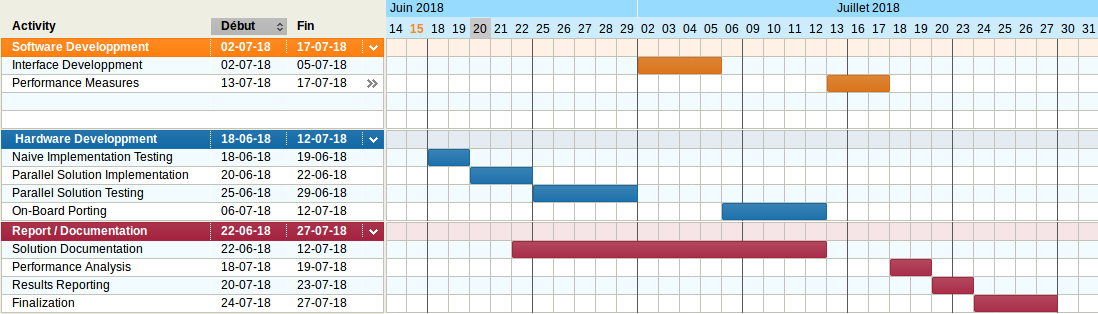
\includegraphics[scale = 0.6, angle = 270]{Figures/new_planif.png}
   \caption{New planification}
    \label{fig:planif}
\end{figure}